% ==========================================
% Section 8: Textual Attributes (Slides 30-38)
% ==========================================

% Slide 30: Text Preprocessing
\begin{frame}{پیش‌پردازش ویژگی‌های متنی}
\begin{columns}[c]
  \begin{column}{0.55\textwidth}
    \begin{itemize}
      \item \textbf{مراحل استاندارد آماده‌سازی متن:}
      \begin{itemize}
        \item \textbf{پاکسازی متن (\lr{Text Cleanup})} حذف علائم نگارشی، تگ‌های \lr{HTML} و کاراکترهای زائد.
        \item \textbf{توکن‌بندی (\lr{Tokenization})} شکستن متن به کلمات منفرد (\lr{Tokens}).
        \item \textbf{تبدیل به حروف کوچک (\lr{Lowercasing}).}
        \item \textbf{حذف کلمات ایست (\lr{Stopwords Removal})} حذف کلمات بسیار رایج فاقد بار اطلاعاتی (مانند حروف اضافه و ربط).
        \item \textbf{ریشه‌یابی و لماتیزاسیون (\lr{Stemming / Lemmatization})} تبدیل واژگان مختلف به ریشه یکسان (مانند \lr{computes, computing $\to$ compute}).
      \end{itemize}
    \end{itemize}
  \end{column}
  \begin{column}{0.43\textwidth}
    \centering
    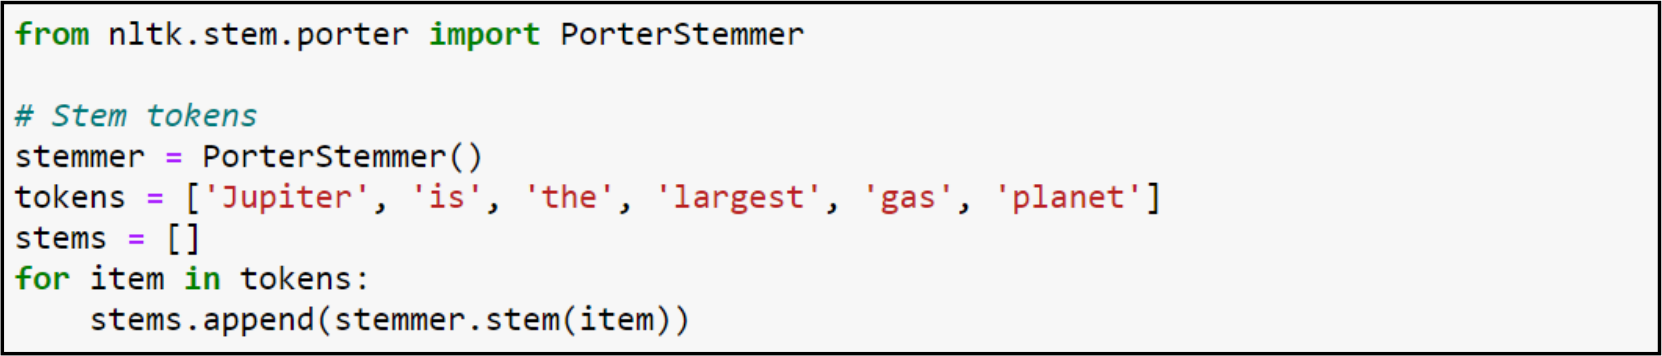
\includegraphics[width=\textwidth]{images/page_30_img_1.png}
  \end{column}
\end{columns}
\end{frame}

% Slide 31: Bag of Words
\begin{frame}{استخراج ویژگی: مدل کیسه کلمات (\lr{Bag-of-Words})}
\begin{columns}[c]
  \begin{column}{0.55\textwidth}
    \begin{itemize}
      \item \textbf{اصول مدل کیسه کلمات (\lr{Bag-of-Words})}
      \begin{itemize}
        \item هر کلمه یکتا در پیکره متنی تبدیل به یک بعد/ویژگی در فضا می‌شود.
        \item ترتیب کلمات و ساختار گرامری جمله نادیده گرفته می‌شود.
        \item هر سند متنی به صورت یک بردار در فضای ویژگی بازنمایی می‌شود.
      \end{itemize}
      \vspace{0.3cm}
      \item مدلی ساده، قدرتمند و بسیار پرکاربرد در بازیابی اطلاعات و دسته‌بندی اسناد.
    \end{itemize}
  \end{column}
  \begin{column}{0.43\textwidth}
    \centering
    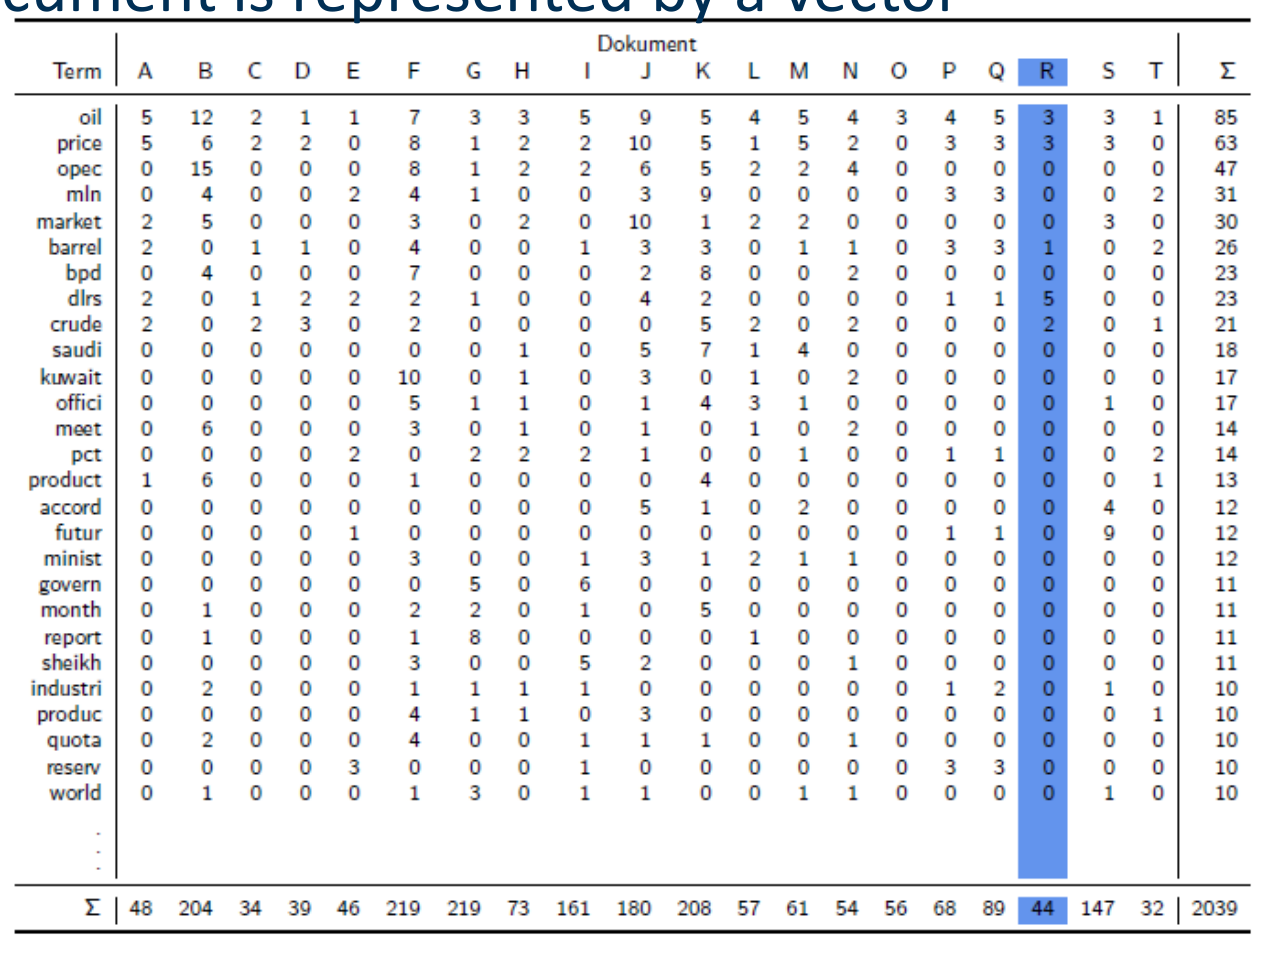
\includegraphics[width=\textwidth]{images/page_31_img_1.png}
  \end{column}
\end{columns}
\end{frame}

% Slide 32: Vector Creation Techniques
\begin{frame}{روش‌های مختلف ساخت بردار ویژگی متنی}
\begin{itemize}
  \item \textbf{تکنیک‌های وزن‌دهی به کلمات درون بردار سند:}
  \begin{itemize}
    \item \textbf{وقوع دودویی کلمه (\lr{Binary Term Occurrence})}
    \begin{itemize}
      \item تنها حضور یا غیبت واژه در سند بررسی می‌شود ($1$ یا $0$) -- نظیر \lr{One-Hot Encoding}.
      \item در پایتون: \codeinline{CountVectorizer(binary=True)}
    \end{itemize}
    \vspace{0.15cm}
    \item \textbf{رخداد و بسامد واژه (\lr{Term Occurrence})}
    \begin{itemize}
      \item تعداد تکرار واژه در سند؛ دارای چالش در صورت متفاوت بودن طول اسناد مختلف.
      \item در پایتون: \codeinline{CountVectorizer(binary=False)}
    \end{itemize}
    \vspace{0.15cm}
    \item \textbf{فراوانی نسبی واژه (\lr{Term Frequency})}
    \begin{itemize}
      \item نسبت تکرار واژه به کل کلمات موجود در همان سند (طول سند).
      \item در پایتون: \codeinline{TfidfVectorizer(use\_idf=False)}
    \end{itemize}
    \vspace{0.15cm}
    \item \textbf{وزن‌دهی \lr{TF-IDF}} (جزئیات و فرمول‌ها در اسلاید بعدی)
    \begin{itemize}
      \item در پایتون: \codeinline{TfidfVectorizer()}
    \end{itemize}
  \end{itemize}
\end{itemize}
\end{frame}

% Slide 33: TF-IDF
\begin{frame}{وزن‌دهی \lr{TF-IDF}}
\begin{itemize}
  \item \textbf{سنجش وزن و اهمیت کلمات با معیار \lr{TF-IDF}}
  \begin{itemize}
    \item کوته‌نوشت \lr{Term Frequency -- Inverse Document Frequency}
    \item ارزیابی اختصاصی بودن یک واژه در یک سند نسبت به کل پیکره متنی:
    $$w_{ij} = tf_{ij} \times idf_i$$
    \item \textbf{بسامد معکوس سند (\lr{IDF})}
    $$idf_i = \log\left(\frac{N}{df_i}\right)$$
    \item $N$: تعداد کل اسناد در پیکره (\lr{Corpus})
    \item $df_i$: تعداد اسنادی که واژه $t_i$ در آن‌ها حداقل یک‌بار ظاهر شده است.
  \end{itemize}
  \vspace{0.15cm}
  \item \textbf{ویژگی کلیدی:}
  \begin{itemize}
    \item اعطای وزن بالاتر به کلمات نادر و تخصصی؛ وزن کمتر به کلمات رایج عمومی.
  \end{itemize}
  \vspace{0.15cm}
  \item \textbf{پیاده‌سازی در \lr{scikit-learn}} (با هموارسازی برای پرهیز از تقسیم بر صفر):
  $$idf_i = \log\left(\frac{1 + N}{1 + df_i}\right) + 1$$
\end{itemize}
\end{frame}

% Slide 34: Similarity of Documents - Jaccard
\begin{frame}{معیارهای شباهت اسناد: ضریب جاکارد (\lr{Jaccard})}
\begin{itemize}
  \item \textbf{معیار شباهت جاکارد (\lr{Jaccard Similarity})}
  \begin{itemize}
    \item معیار شباهت برای بردارهایی با ویژگی‌های دودویی نامتقارن (\lr{Asymmetric Binary})
    $$\text{Jaccard}(A, B) = \frac{|A \cap B|}{|A \cup B|} = \frac{M_{11}}{M_{01} + M_{10} + M_{11}}$$
  \end{itemize}
  \vspace{0.2cm}
  \item \textbf{کاربرد در کنار بردارهای وقوع دودویی (\lr{One-Hot Vectors})}
  \begin{itemize}
    \item مقدار ۱ نشان‌دهنده حضور واژه در سند است.
    \item مقدار ۰ نشان‌دهنده غیبت واژه در سند است.
    \item در بیشتر اسناد، اکثر مقادیر صفر هستند چون هر سند تنها از بخش ناچیزی از کل دایره واژگان استفاده می‌کند.
    \item غیبت مشترک واژه‌ها ($M_{00}$) نباید نقشی در افزایش شباهت دو متن داشته باشد!
  \end{itemize}
\end{itemize}
\end{frame}

% Slide 35: Jaccard Calculation Example
\begin{frame}{محاسبه ضریب جاکارد: مثال عملی}
\centering
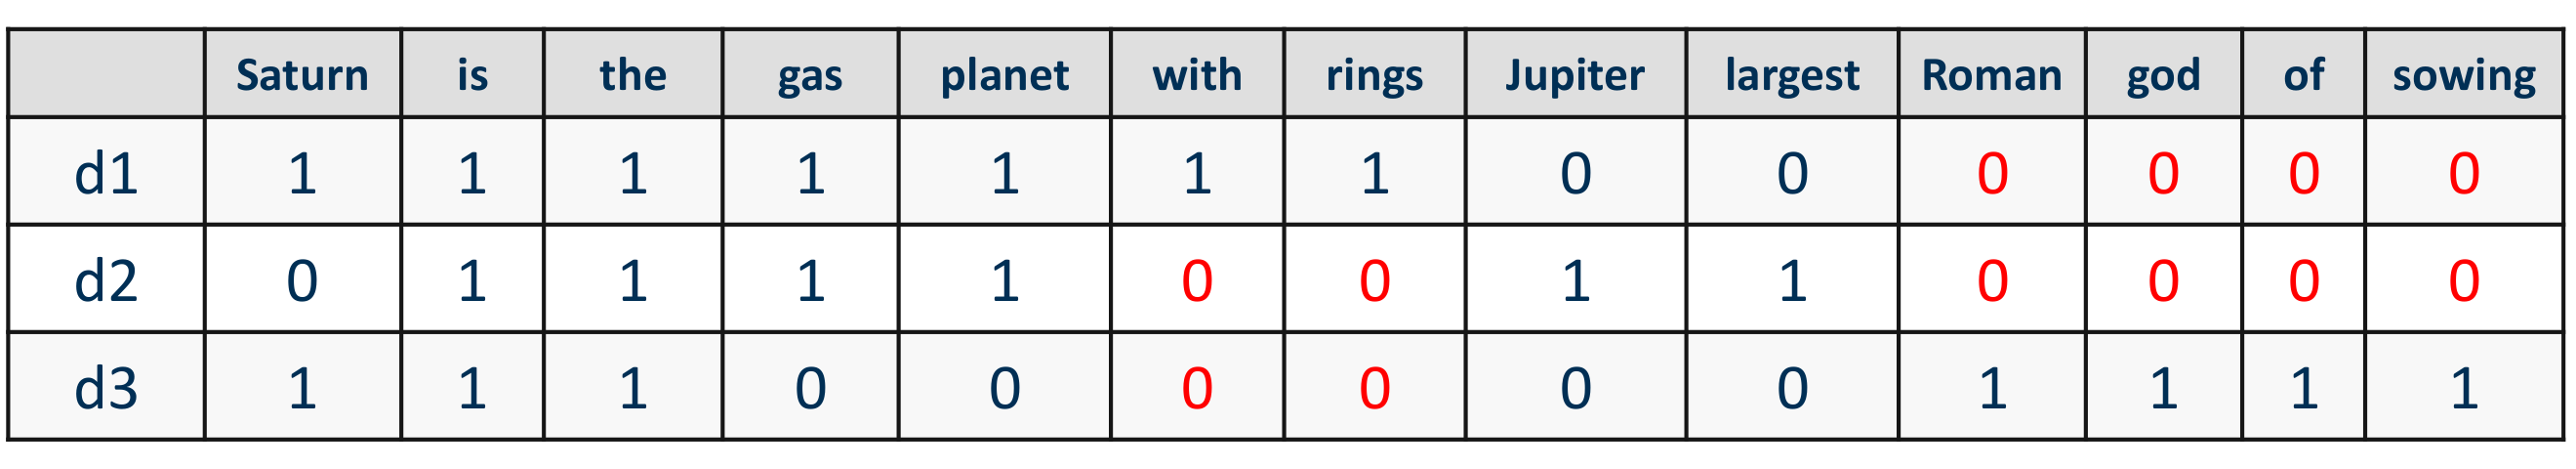
\includegraphics[width=0.95\textwidth]{images/page_35_table.png}
\vspace{0.3cm}
\begin{itemize}
  \item \textbf{محاسبه شباهت‌های جاکارد بین اسناد سه‌گانه:}
  \begin{itemize}
    \item $\text{Jaccard}(d_1, d_2) = \frac{4}{9} \approx 0.44$
    \item $\text{Jaccard}(d_2, d_3) = \frac{2}{11} \approx 0.18$
    \item $\text{Jaccard}(d_1, d_3) = \frac{3}{11} \approx 0.27$
  \end{itemize}
\end{itemize}
\end{frame}

% Slide 36: Cosine Similarity
\begin{frame}{معیار شباهت کسینوسی (\lr{Cosine Similarity})}
\begin{itemize}
  \item \textbf{شباهت کسینوسی (\lr{Cosine similarity})}
  \begin{itemize}
    \item معیار شباهت برای مقایسه بردارهای وزنی سند (مانند بردار بسامد یا \lr{TF-IDF})
    $$\cos(d_1, d_2) = \frac{d_1 \cdot d_2}{\|d_1\| \, \|d_2\|}$$
    \item که در آن $\cdot$ نشان‌دهنده ضرب داخلی بردارها ($a \cdot b = \sum_{i=1}^n a_i b_i$) و $\|d\|$ طول بردار ($\|d\| = \sqrt{\sum_{i=1}^n d_i^2}$) است.
  \end{itemize}
  \item \textbf{مثال عددی (\lr{Example})}
  \begin{itemize}
    \item $d_1 = (3, 2, 0, 5, 0, 0, 0, 2, 0, 0) \qquad d_2 = (1, 0, 0, 0, 0, 0, 0, 1, 0, 2)$
    \item $d_1 \cdot d_2 = 3\times 1 + 2\times 0 + 0\times 0 + 5\times 0 + \dots + 2\times 1 + 0\times 0 + 0\times 2 = 5$
    \item $\|d_1\| = (3^2 + 2^2 + 0^2 + 5^2 + 0^2 + 0^2 + 0^2 + 2^2 + 0^2 + 0^2)^{0.5} = \sqrt{42} \approx 6.481$
    \item $\|d_2\| = (1^2 + 0^2 + 0^2 + 0^2 + 0^2 + 0^2 + 0^2 + 1^2 + 0^2 + 2^2)^{0.5} = \sqrt{6} \approx 2.245$
    \item $\cos(d_1, d_2) = \frac{5}{6.481 \times 2.245} = \frac{5}{14.549} \approx 0.3150$
  \end{itemize}
\end{itemize}
\end{frame}

% Slide 37: Dense and Sparse Representation
\begin{frame}{بازنمایی‌های چگال و خلوت (\lr{Dense and Sparse})}
\begin{columns}[c]
  \begin{column}{0.55\textwidth}
    \begin{itemize}
      \item \textbf{کیسه کلمات خلوت (\lr{Sparse}) است:}
      \begin{itemize}
        \item ابعاد بردار در حد ده‌ها هزار است.
        \item بیشتر درایه‌ها صفر هستند.
      \end{itemize}
      \vspace{0.3cm}
      \item \textbf{بازنمایی چگال (\lr{Dense representation}):}
      \begin{itemize}
        \item تعبیه کلمات (\lr{Word embeddings})
        \item برداری با ابعاد چند صدتایی
      \end{itemize}
    \end{itemize}
  \end{column}
  \begin{column}{0.43\textwidth}
    \centering
    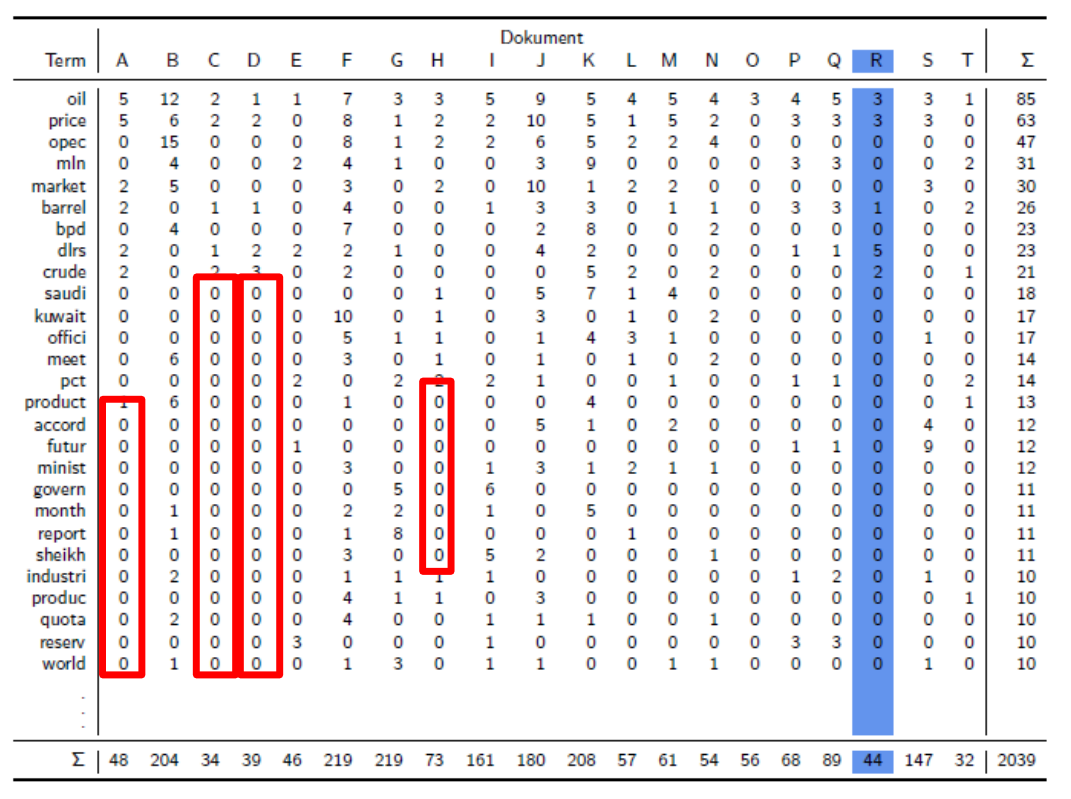
\includegraphics[width=\textwidth]{images/page_37_img_1.png}
  \end{column}
\end{columns}
\end{frame}

% Slide 38: Transformer Architecture
\begin{frame}{معماری ترنسفورمر (\lr{Transformer Architecture})}
\begin{columns}[c]
  \begin{column}{0.55\textwidth}
    \begin{itemize}
      \item \textbf{فقط رمزگذار (\lr{Encoder-only}):}
      \begin{itemize}
        \item \lr{BERT}، \lr{ALBERT}، \lr{RoBERTa}
      \end{itemize}
      \vspace{0.2cm}
      \item \textbf{فقط رمزگشا (\lr{Decoder-only}):}
      \begin{itemize}
        \item مدل‌های زبانی بزرگ مانند \lr{GPT}، \lr{LLaMA} و ...
      \end{itemize}
      \vspace{0.2cm}
      \item \textbf{دنباله به دنباله (\lr{Seq2Seq}):}
      \begin{itemize}
        \item \lr{T-5} (\lr{Text-to-Text Transfer Transformer})
        \item \lr{BART}
      \end{itemize}
    \end{itemize}
  \end{column}
  \begin{column}{0.43\textwidth}
    \centering
    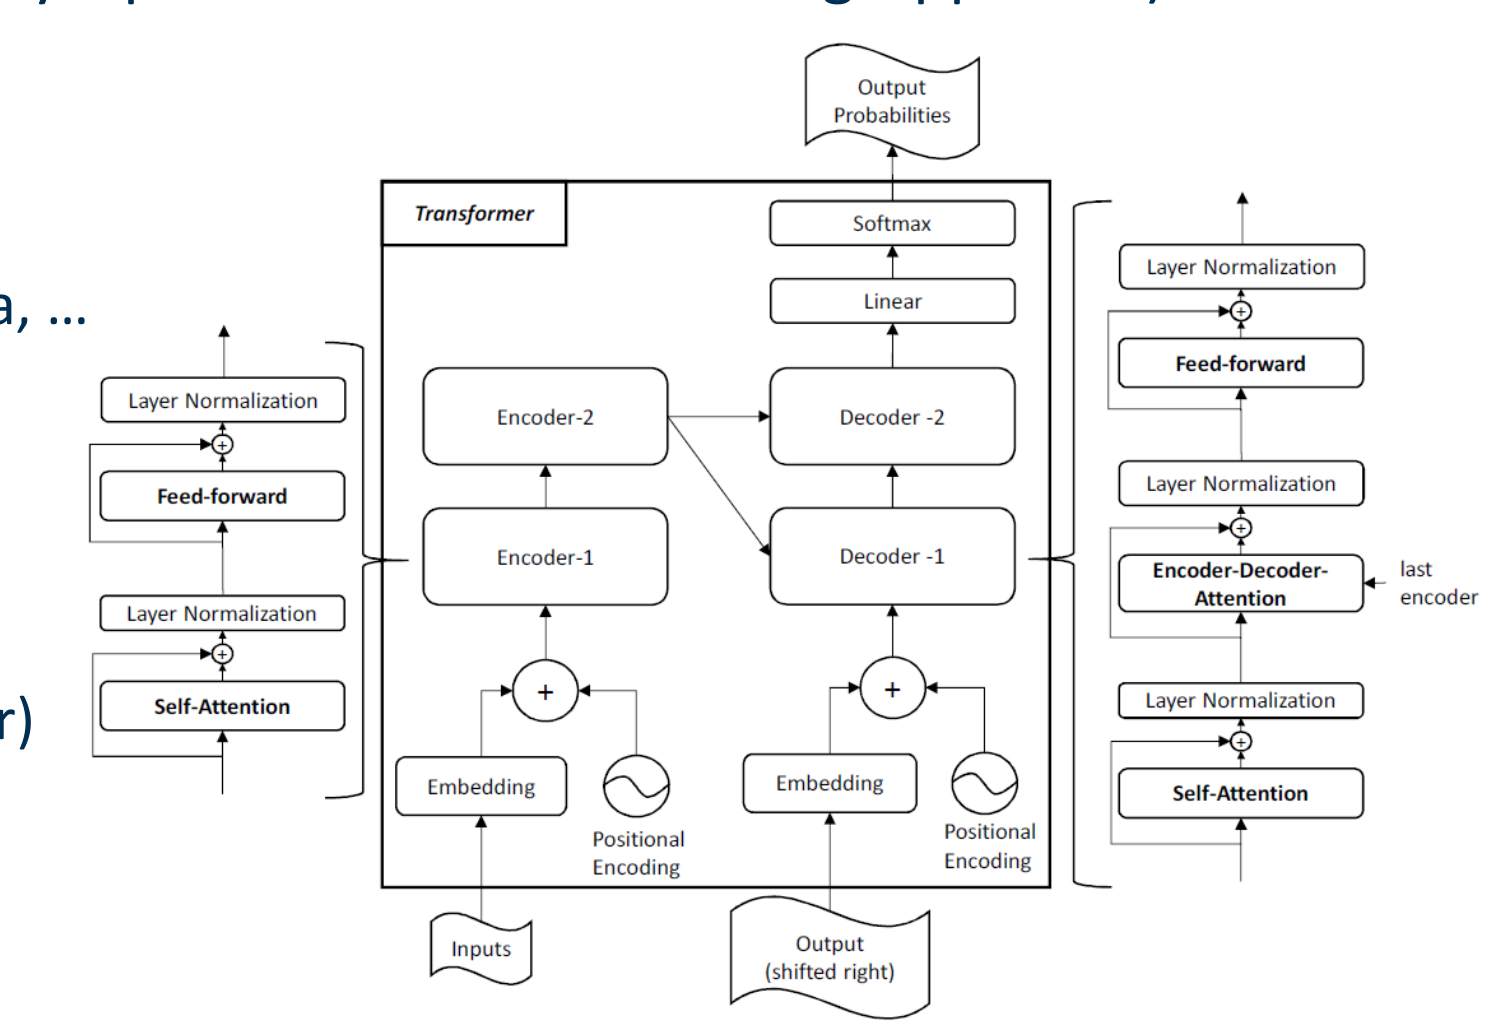
\includegraphics[width=\textwidth]{images/page_38_img_1.png}
  \end{column}
\end{columns}
\end{frame}
